\begin{quote}
	\textbf{Abstract:} 
\end{quote}

\section{Introduction}
Continuous technological advancements to high-throughput profiling of single cells
are having profound effects on how researchers can validate biological hypotheses. 
For example, single-cell RNA sequencing (scRNA-seq) directly resulted in the development
of a new type of computational method called trajectory inference (TI). By profiling
the transcriptomics profiles of developing cells, TI methods attempt to reconstruct 
and characterise the underlying dynamic processes \cite{cannoodt_computationalmethodstrajectory_2016}.
While early experimental technologies allowed to profile one single modality (e.g. DNA sequence, 
RNA or protein expression), recent developments permit profiling multiple modalities simultaneously.

An ideal experiment would be able to observe all aspects of a cell, including a full history of its 
molecular states, spatial positions and environmental interactions \cite{stuart_integrativesinglecellanalysis_2019}. 
While this falls outside the reach of current experimental technologies, \textit{in silico} simulations
of single cells would allow developing the next wave of computational techniques
in anticipation of new experimental technologies.

A few generators of scRNA-seq profiles have already been developed (e.g. splatter \cite{zappia_splattersimulationsinglecell_2017}, powsimR \cite{vieth_powsimrpoweranalysis_2017} and PROSSTT \cite{papadopoulos_prossttprobabilisticsimulation_2018}). % BoolODE and dyntoy are also examples.
These can be used to evaluate the performance of computational tools, and to explore their strengths and weaknesses. A limitation of directly simulating a scRNA-seq profile (instead of a single cell) is that extending the simulation to other aspects of the cell -- such as tracking the full history of molecular states -- becomes difficult.

We introduce dyngen, a multi-modality simulator of single cells (Figure \ref{fig:dyngen}).
dyngen was initially developed as part of a comprehensive benchmark of TI methods \cite{saelens_comparisonsinglecelltrajectory_2019} but has since been extended to be applicable in a much broader context.

Inspiration was drawn from GeneNetWeaver's \cite{schaffter_genenetweaversilicobenchmark_2011} workflow to generate \textit{in silico} bulk profiles for evaluating network inference methods \cite{marbach_wisdomcrowdsrobust_2012}. GeneNetWeaver translates a known gene regulatory network (GRN) into sets of Ordinary Differential Equations (ODE) in order to simulate \ldots. % todo: describe GNW in this one sentance
There are two significant differences in dyngen in comparison to GeneNetWeaver. 
dyngen simulates a single-cell instead of a bulk profile. However, taking random walks through ODE systems in which key molecules occur with low abundance can result in inaccurate results. %rephrase and cite relevant work
Gillespie's Stochastic Simulation Algorithm (SSA)  \cite{gillespie_exactstochasticsimulation_1977} allows to simulate low abundance systems.
Running a simulation with SSA is an iterative process where at each iteration one reaction is allowed to take place. Each reaction consists of its propensity -- a formula to calculate the probability of occurring during an infinitesimal time interval -- and the effect -- how it will affect the current state if triggered.
Secondly, the GRN is constructed such that it mimics a dynamic process of interest, such as cell differentiation into multiple cell types. 

We demonstrate dyngen's flexibility by simulating numerous different types of biological experiments, and using these simulations to develop new benchmarking techniques for computational tools.

\begin{figure}[htb!]
	\centering
	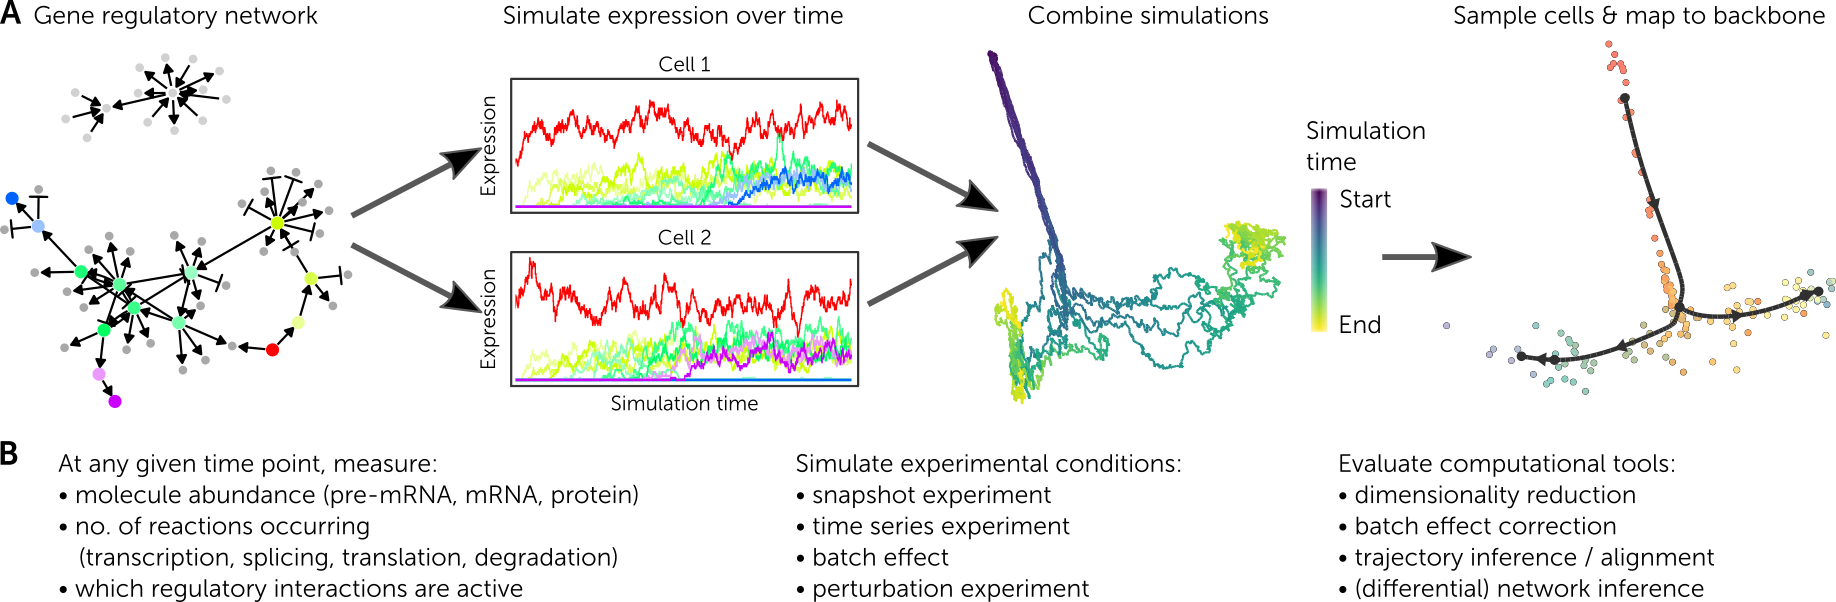
\includegraphics[width=\linewidth]{fig/showcase_3.png} 
	\caption{Showcase of dyngen functionality. \textbf{TODO: change to pdf.} Remove B?} % TODO: update label
	\label{fig:dyngen}
\end{figure}

\section{Results}
dyngen is a simulator for single cells that develop over time. Throughout this section, a simple simulation of a cell undergoing a cyclic process is used to illustrate key strengths of dyngen (Figure \ref{fig:simplecyclic}). This example only comprises of a single cell containing 5 genes, but dyngen can easily scale up to thousands of simulations containing thousands of genes.

\begin{figure}[htb!]
	\centering
	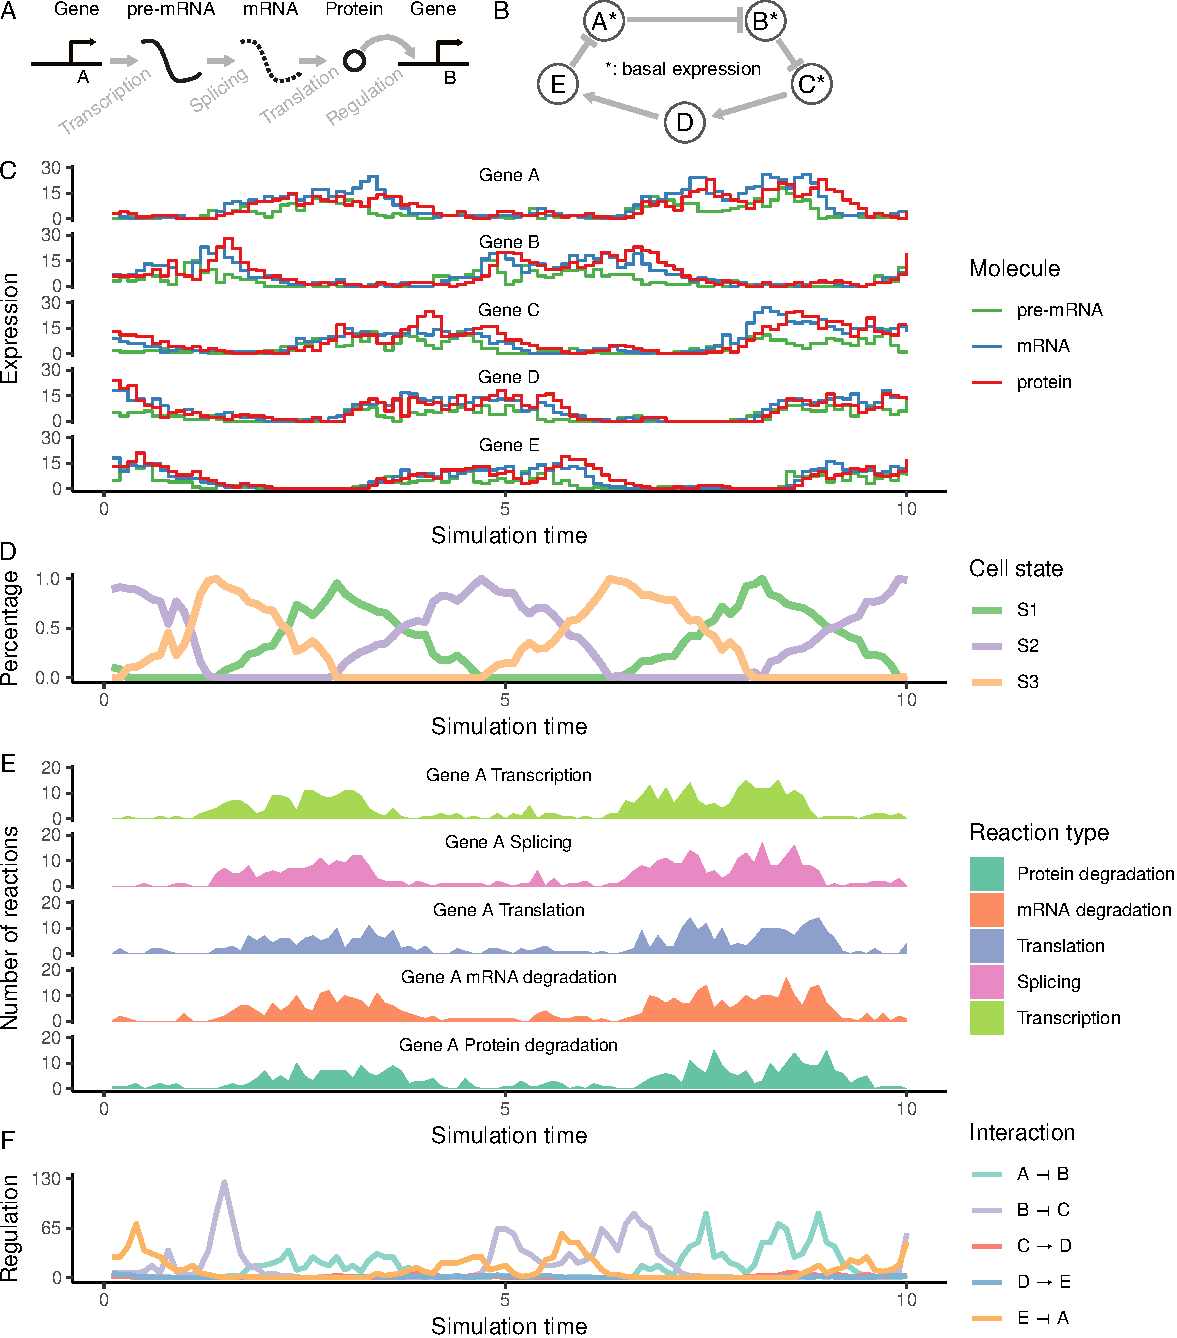
\includegraphics[width=\linewidth]{fig/simplecyclic_edited} 
	\caption{Showcase of dyngen functionality. A time resolution of 0.1 was used, but this can be increased or decreased without effect on performance of the execution of the simulation. \textbf{TODO: perhaps it's better to replace Figure \ref{fig:simplecyclic} with one subfigure for each of the paragraphs in this text.}}
	\label{fig:simplecyclic}
\end{figure}

In dyngen, a cell consists of a set of molecules, the abundance of which are affected by a set of reactions: transcription, splicing, translation, and degradation (Figure \ref{fig:simplecyclic}A). These reactions are determined from a predefined set of gene regulatory interactions (Figure \ref{fig:simplecyclic}B), henceforth referred to as a gene regulatory network (GRN). The likelihood of a reaction occurring at any given point in time is defined by the GRN and by the abundance of molecules involved each reaction.

One of dyngen's main advantages is that through careful engineering of the GRN, different cellular developmental processes can be obtained. Different GRNs can result in branching, converging, cyclic, or even disconnected developmental topologies. Multiple simulations with slightly different GRNs can emulate rewiring events in disease or perturbation experiments. % could use figure; one with GRNs of different topologies, another with rewiring events
Multiple simulations with different initial molecule abundance levels can be used to replicate batch effects. 

Another advantage is that dyngen returns many modalities throughout the whole simulation: molecular abundance, cellular state, number of reaction firings, reaction likelihoods, and regulation activations (Figure \ref{fig:simplecyclic}C--F). These modalities can serve both as input data and ground truth for benchmarking many types of computational approaches. For example, a network inference method could use mRNA abundance and cellular states as inputs, and its output could be benchmarked against the gold standard GRN.

The final main advantage is that by making alterations to the simulation pipeline, multiple types of experiments (sampling technique or profiling technique) can be simulated. By default, dyngen supports snapshot experiments (uniformly sampling from an asynchronous dynamic process) and time-series experiments (sampling cells from different intervals in the simulation). 
It is possible to implement other experimental protocols (which perhaps do not exist in real life), such as sampling the same cell at regular intervals. 

%% TODO: show that dyngen output resembles real data using e.g. countsimQC?

%% TODO: add result figures pertaining use cases

\section{Discussion}
As is, dyngen's single cell simulations can be used to evaluate common single-cell omics computational methods such as clustering, batch correction, trajectory inference and network inference.
However, the combined effect of these advantages results in a framework that is flexible enough to adapt to a broad range of applications. This may include methods that integrate clustering, network inference and trajectory inference. In this respect, dyngen may promote the development of new tools in the single-cell field similarly as other simulators have done in the past \cite{schaffter_genenetweaversilicobenchmark_2011,ewing_combiningtumorgenome_2015}.

Adding batch effects to snapshot simulations of linear (or even branching) trajectories allows evaluating trajectory alignment methods -- which attempt to map two or more trajectories onto each other. Adding perturbations to the GRN allows evaluating the performance of differential network inference methods -- which predict differential regulatory interactions between two or more groups of profiles.  Sampling a cell at a particular time point and once more at a later time point allows evaluating the performance of RNA velocity approaches -- which predict the future state of a cell by looking at differences in pre-mRNA and mRNA abundance levels.

dyngen ultimately also allows anticipating technological developments in single-cell multi-omics. In this way, it is possible to design and evaluate the performance and robustness of new types of computational analyses before experimental data becomes available.
Similarly, it could also be used to compare which experimental technique will likely produce the most accurate result. For example, is it possible to infer directionality of regulatory interactions from snapshot experiments only, or are time series or knockdown experiments a necessity in order to infer high-quality regulatory networks?

Currently, dyngen focuses on simulating cells as standalone entities.
Future developments include extending the framework to simulate multiple cells in a virtual environment. Allowing cells to receive and react to environmental and intercellular stimuli would enable simulating essential cellular processes such as cell division and migration. 
%¡also adding more types of molecules, e.g. protein complex, small rnas, PPI
\section{Methods}
NOTE: The method section is really rough at this stage.

The workflow to generate \textit{in silico} single cell data consists of six main steps (Figure \ref{fig:explain_methods}). 

\begin{figure}[htb!]
	\centering
	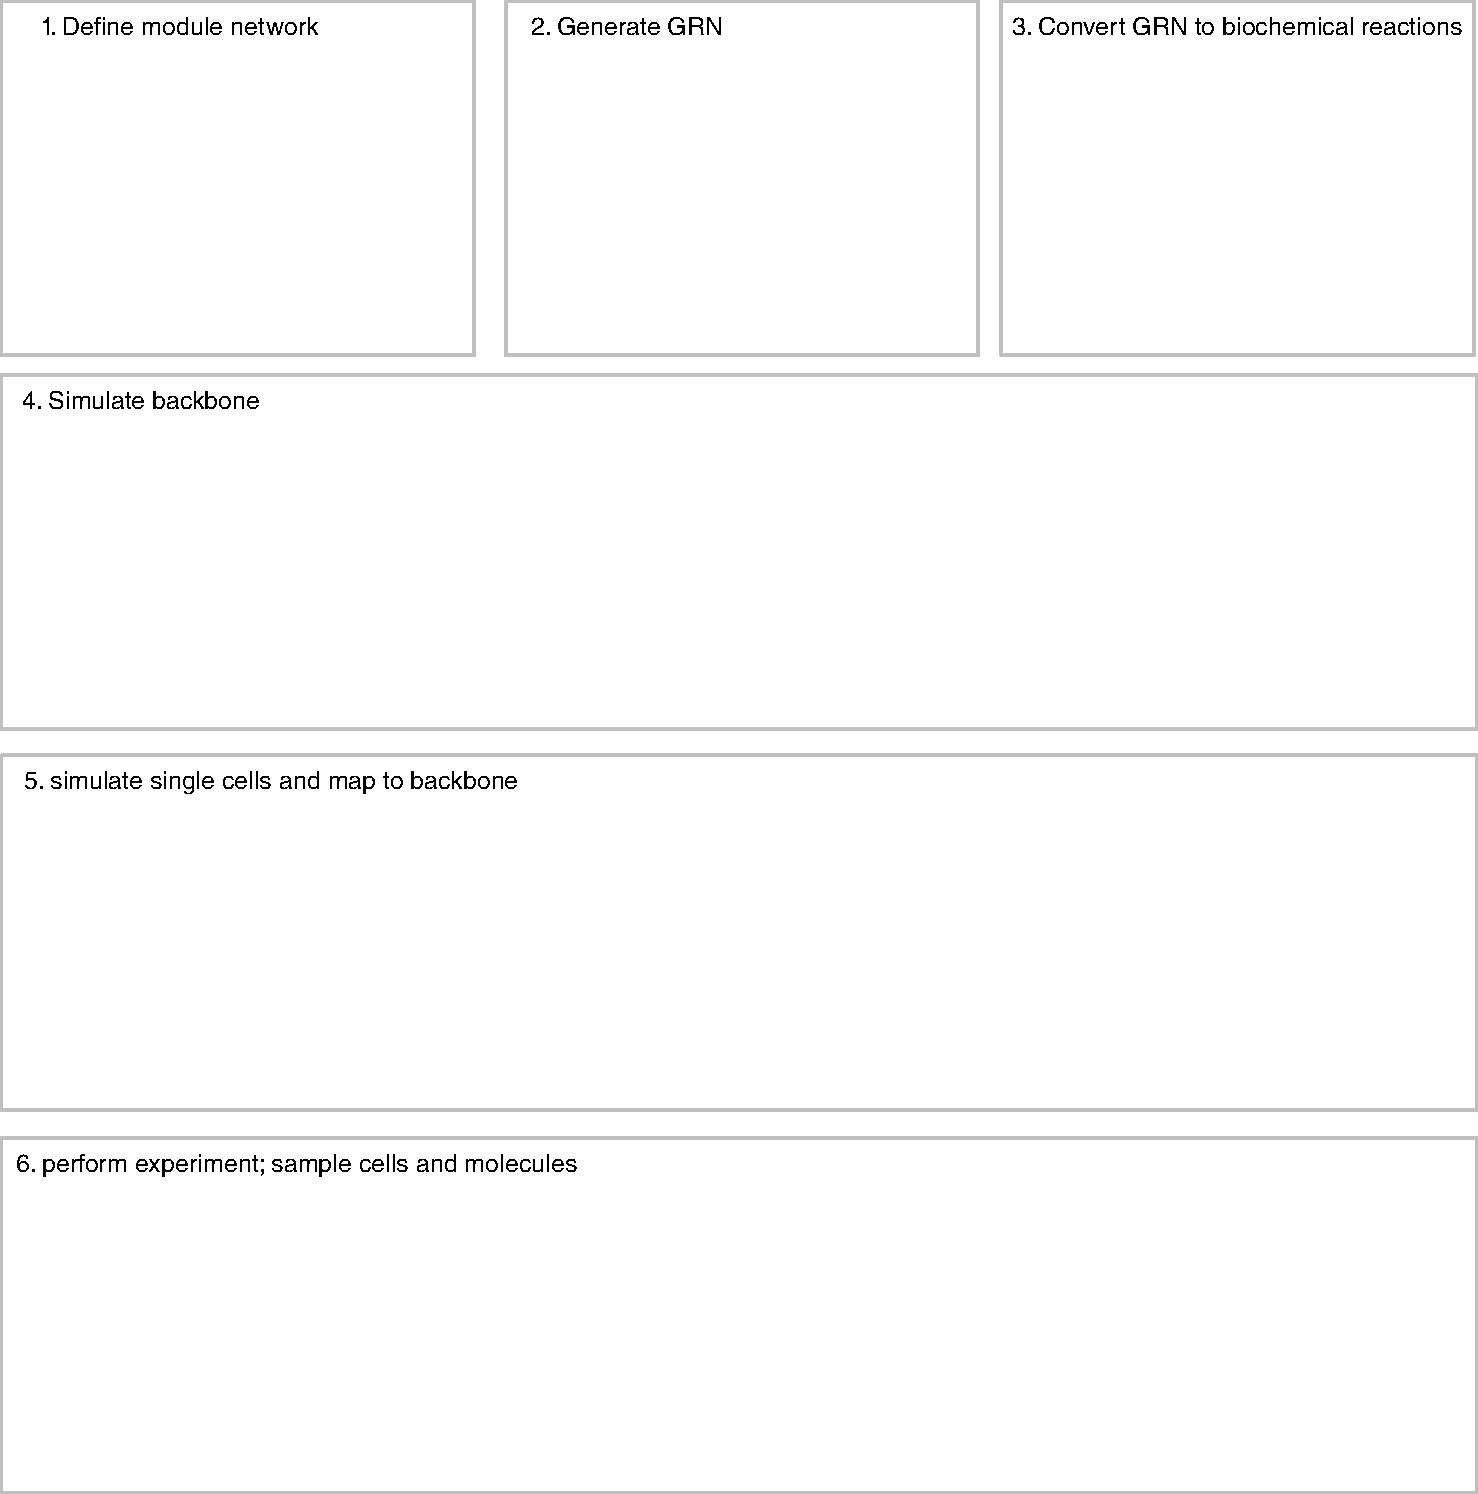
\includegraphics[width=\hugefigure]{fig/explain_methods} 
	\caption{\textbf{The workflow of dyngen is comprised of six main steps.} \textbf{A:} The user needs to specify the desired module network or use a predefined module network. \textbf{B:} Each gene in a module is is regulated by one or more transcription factors from the upstream module. Additional target genes are generated. \textbf{C:} Each gene regulatory interaction in the GRN is converted to a set of biochemical reactions. \textbf{D:} Along with the module network, the user also needs to specify the backbone structure of expected cell states. The average expression of each edge in the backbone is simulated by activating a restricted set of genes for each edge. \textbf{E:} Multiple Gillespie SSA simulations are run using the reactions defined in step C.  The counts of each of the mocules at each time step are extracted. Each time step is mapped to a point in the backbone. \textbf{F:} Multiple cells are sampled from each simulation. Molecules are sampled from each cell.}
	\label{fig:explain_methods}
\end{figure}

\subsection{Defining the backbone: modules and states} \label{sec:backbone}

One of the main processes involved in cellular dynamic processes is gene regulation, where regulatory cascades and feedback loops lead to progressive changes in expression and decision making. The exact way a cell chooses a certain path during its differentiation is still an active research field, although certain models have already emerged and been tested \textit{in vivo}. One driver of bifurcation seems to be mutual antagonism, where two genes \cite{xu_regulationbifurcatingcell_2015} strongly repress each other, forcing one of the two to become inactive \cite{graf_forcingcellschange_2009}. Such mutual antagonism can be modelled and simulated \cite{wang_quantifyingwaddingtonlandscape_2011, ferrell_bistabilitybifurcationswaddington_2012}. Although the two-gene model is simple and elegant, the reality is frequently more complex, with multiple genes (grouped into modules) repressing each other \cite{yosef_dynamicregulatorynetwork_2013}.

In dyngen, the user defines the behaviour of the simulation by defining how sets of genes, called modules, are regulating eachother.
A module may have basal expression, which means that pre-mRNA of the genes in this module will be transcribed without the presence of transcription factor molecules. A module marked as "active during the burn phase" means that this module will be allowed to generate expression of its genes during an initial warm-up phase (See section \ref{sec:dyngen_ssa}). At the end of the dyngen process, cells will not be sampled from the burn phase simulations.

Several examples of module networks are given (Figure \ref{fig:example_backbones}). 
A simple chain of modules (where one module upregulates the next) results in a \emph{linear} process. By having the last module repress the first module, the process becomes \emph{cyclic}. Two modules repressing eachother is the basis of a \emph{bifurcating} process, though several chains of modules have to be attached in order to achieve progression before and after the bifurcation process. Finally, a \emph{converging} process has a bifurcation occurring during the burn phase, after which any differences in module regulation is removed.

Note that these examples represent the bare minimum in terms of number of modules used. Using longer chains of modules is typically desired. In addition, the fate decisions made in this example of a bifurcation is reversible, meaning cells can be reprogrammed to go down a different differentiation path. If this effect is undesirable, more safeguards need to be put in place to prevent reprogramming from occurring (Section \ref{sec:dyngen_backbone_lego}).

TODO: mention strength and cooperativity.

\begin{figure}[htb!]
	\centering
	\includegraphics[width=\LARGEfigure]{fig/example_backbones} 
	\caption{Example module networks}
	\label{fig:example_backbones}
\end{figure}

In addition to the module network, the user also needs to define a network of cellular states called the "backbone". Before simulating any cells, each transition in the backbone is simulated separately to obtain the average changes in expression along that transition (Figure \ref{fig:explain_methods}D). As part of the backbone, the user needs to specify which modules are allowed to alter its expression from one state to another. For example, in order to transition from state S0 to S1 in the cyclic example, gene modules A, B and C are turned on and a simulation is allowed to run. To transition from S1 to S2, gene modules D and E are turned on, and expression of gene module C is kept constant. To transition from S2 to S3, C is turned on again and now A and B are fixed. Finally, to transition from S3 to S1 again, A and B are turned on again and D and E are fixed again. Demonstrations of the backbone will be explained in more detail in section \ref{sec:dyngen_sim_backbone}.

\subsubsection{Backbone lego} \label{sec:dyngen_backbone_lego}
The backbone can make use of one or more "backbone lego" (BBL) pieces (Figure \ref{fig:backbone_lego}). A BBL consists of one or more modules which regulate each other such that the output modules present a specific behaviour, depending on the input module (Figure \ref{fig:backbone_lego}A). Parameters allow determining the number of modules involved in the process and the number of outputs. Multiple BBLs can be chained together in order to intuitively create milestone networks and corresponding state networks (Figure \ref{fig:backbone_lego}B). Note that not all dynamic processes can be represented by a combination of BBLs, but they can serve as common building blocks to aid the construction of the backbone.

\begin{figure}[htb!]
	\centering
	\includegraphics[width=\LARGEfigure]{fig/backbone_lego} 
	\caption{Backbone lego}
	\label{fig:backbone_lego}
\end{figure}

When the input node of a \textbf{linear BBL} (Figure \ref{fig:backbone_lego}C) is upregulated, the module the BBL is connected to will be upregulated. A \emph{simple chain} is a set of modules where a module upregulates the next. A \emph{chain with double repression} has an uneven number of modules forming a chain where each module downregulates the next but all modules (except the input) have basal expression. A \emph{grid with double repression} is similar; except that modules do not have basal expression but instead get upregulated by an upstream module in the chain. Finally, a \emph{flip flop} consists of a simple chain where first the modules (except the last) are upregulated. Once the second to last module is upregulated, that module upregulates itself and the first module is strongly repressed, causing all other modules to lose expression and finally the last module to be upregulated. The \emph{flip flop} retains this output state, even when the input changes.

When the input node of a \textbf{branching BBL} (Figure \ref{fig:backbone_lego}D) is upregulated, a subset of its output modules will eventually be upregulated. A \emph{simple branching} uses reciprocal inhibition to drive the upregulation of one of the output modules. Due to its simplicity, however, multiple output modules might be upregulated simultaneously, and over long periods of simulation time it might be possible that the choice of upregulated module changes. A \emph{robust branching} improves upon the simple branching by preventing upregulation of output modules until an internal branching decision has been made, and by repressing the decision mechanism to avoid other output modules being upregulated other than the one that has been chosen.

A \textbf{leaf BBL} (Figure \ref{fig:backbone_lego}E) is a linear BBL that has either no inputs or no outputs. A \emph{start} BBL is a linear BBL where the first module has basal expression, and all modules in this module will be active during the burn-in phase of the simulation (Section \ref{sec:dyngen_sim_backbone}). An \emph{end} BBL is also a linear BBL with its output regulating one final module. 


\subsection{Generate gene regulatory network}
% TODO: write section in words instead of bullet point list

\subsubsection{Generate the transcription factor network}
Parameters: 
\begin{itemize}
	\item Number of TFs to generate $num\_tfs$
	\item Minimum TFs per module $min\_tfs$, default = 1
	\item Number of regulatory interactions per module interaction $num\_tf\_ints$, default = 2
\end{itemize}

Procedure: 
\begin{itemize}
	\item Divide $num\_tfs$ TFs amongst modules in backbone such that each module has at least $min\_tfs$ TFs.
	\item For every TF in a particular module $M$, connect that TF with $num\_tf\_ints$ TFs for each upstream module of $M$.
	\item The strength and cooperativity of interactions created this way are defined by the module network.
\end{itemize}

\subsubsection{Generate targets}
Parameters: 
\begin{itemize}
	\item Number of target genes $num\_targets$
	\item Name of a FANTOM5 GRN
	\item Damping factor $damping$, default = 0.05
	\item Target resampling $resamp$, default = $+\infty$
	\item Maximum in-degree $max\_in\_degree$, default = 5
\end{itemize}

Procedure:
\begin{itemize}
	\item Download the FANTOM5 GRN if not already available
	\item Randomly map TFs to the regulators in the GRN
	\item Compute page rank from the selected regulators in the GRN with damping factor $damping$
	\item Perform weighted sample of  $\min(num\_targets, resamp)$ targets weighted by the page rank
	\item Select subgraph induced by the TFs and the sampled targets in the GRN, remove edges to the TFs
	\item Add subgraph to current TF-target network
	\item If less than $num\_targets$ have been sampled in this way, go back to step 2.
	\item Remove regulatory interactions if a target has more than $max\_in\_degree$ edges.
\end{itemize}

\subsubsection{Generate housekeeping genes}
Parameters: 
\begin{itemize}
	\item Number of housekeeping genes $num\_targets$
	\item Name of a FANTOM5 GRN
	\item Target resampling $resamp$, default = $+\infty$
	\item Maximum in-degree $max\_in\_degree$, default = 5
\end{itemize}

Procedure:
\begin{itemize}
	\item Use same FANTOM5 GRN
	\item Subsample GRN such that each gene has a maximum in-degree of $max\_in\_degree$
	\item Perform breadth-first-search from a random gene in the GRN, select $\min(num\_targets, resamp)$ first genes encountered
	\item Select subgraph induced by the sampled housekeeping genes in the GRN
	\item Add subgraph to current TF-target network
	\item If less than $num\_targets$ have been sampled in this way, go back to step 2.
\end{itemize}

\subsection{Convert gene regulatory network to a set of reactions} \label{sec:reactions}
% TODO: write section in words instead of bullet point list

Each reaction consists of its propensity -- a formula to calculate the probability of occurring during an infinitesimal time interval -- and the effect -- how it will affect the current state if triggered.


\newcommand{\w}[1]{\text{w}_{#1}}
\newcommand{\x}[1]{\text{x}_{#1}}
\newcommand{\y}[1]{\text{y}_{#1}}


\newcommand{\rs}[1]{\text{R}_{#1}}
\newcommand{\rp}[1]{\text{R}^+_{#1}}
\newcommand{\rn}[1]{\text{R}^-_{#1}}

\newcommand{\wpr}[1]{\text{wpr}_{#1}}
\newcommand{\wsr}[1]{\text{wsr}_{#1}}
\newcommand{\xdr}[1]{\text{xdr}_{#1}}
\newcommand{\ypr}[1]{\text{ypr}_{#1}}
\newcommand{\ydr}[1]{\text{ydr}_{#1}}

\newcommand{\str}[1]{\text{str}_{#1}}
\newcommand{\co}[1]{\text{co}_{#1}}
\newcommand{\ind}[1]{\text{ind}_{#1}}
\newcommand{\hmy}[1]{\text{hmy}_{#1}}
\newcommand{\reg}[1]{\text{reg}_{#1}}
\newcommand{\ba}[1]{\text{ba}_{#1}}

We define the abundance levels of pre-mRNA, mRNA and protein of gene $G$ as $\w G$, $\x G$ and $\y G$ respectively. Five reactions affect the abundance levels of these molecules: transcription, splicing, mRNA degradation, translation, and protein degradation. The effects and propensity functions of these reactions are defined in Table \ref{tab:reaction_def}.

% see https://en.wikipedia.org/wiki/Hill_equation_(biochemistry)#Regulation_of_gene_transcription
\begin{table}[h]
	\caption{\textbf{Reactions affecting the abundance levels of pre-mRNA $\w G$, mRNA $\x G$ and proteins $\y G$ of gene $G$.} Define the set of regulators of $G$ as $\rs{G}$, the set of upregulating regulators of $G$ as $\rp G$, and the set of downregulating regulators of $G$ as $\rn G$. Parameters used in the propensity formulae are defined in Table \ref{tab:reaction_params}.} \label{tab:reaction_def}
	\centering
	\begin{tabular}{|lcc|}
		\hline
		Reaction & Effect & Propensity \\ \hline \hline
		Transcription & $\emptyset \rightarrow \w G$ & $\wpr G \times \frac{\ba G - \ind{G}^{|\rp{G}|} + \prod\limits_{H \in \rp{G}}(\ind G + \reg{G,H})}{\prod\limits_{H \in \rp{G}}(1 + \reg{G,H})}$ \\
		Splicing & $\w G \rightarrow \x G$ & $\wsr G \times \w G$ \\
		mRNA degradation & $\x G \rightarrow \emptyset$ & $\xdr G \times \x G$ \\
		Translation & $\x G \rightarrow \w G + \y G$ & $\ypr G \times \x G$ \\
		Protein degradation & $\y G \rightarrow \emptyset$ & $\ydr G \times \y G$ \\ \hline
	\end{tabular}
\end{table}

% TODO: explain derivation of transcription formula? 
% regG,H represents a 'probability' that H is bound to G (though does not yet scale between [0,1]). y_H / maxy_H is more likely to be a probability that H is bound to G, though this does not take into account that H can be bound to other genes as well. 
% in any case, if it is, then it upregulates G by strG,H. It is assumed binding events
% are independent and result in multiplicative effect.

% according to https://en.wikipedia.org/wiki/Hill_equation_(biochemistry)#Proportion_of_ligand-bound_receptors:
% P_H = (y_H ^ N) / (degradation_H / production_H + y_H ^ N)
% ... 
% ... 
% might need to go back to things like:
% https://kar.kent.ac.uk/24077/1/myzabetpaper.pdf

\begin{table}[h]
	\caption{\textbf{Parameters defined for the calculation of reaction propensity functions.}} \label{tab:reaction_params}
	\centering
	\begin{tabular}{|lrl|}
		\hline
		Parameter & Symbol & Definition \\ \hline \hline
		Transcription rate & $\wpr{G}$ & $\in N(100, 20),\ \geq 10$ \\
		Splicing rate & $\wsr G$ & $\in N(10, 2),\ \geq 2$ \\
		mRNA degradation rate & $\xdr{G}$ & $\in N(5, 1),\ \geq 2$ \\
		Translation rate & $\ypr{G}$ & $\in N(5, 1),\ \geq 2$ \\
		Protein degradation rate & $\ydr G$ & $\in N(3, 0.5),\ \geq 1$ \\
		Interaction strength & $\str{G,H}$ & $\in 10^{U(0, 2)}$ * \\ 
		Interaction cooperativity & $\co{G,H}$ & $\in U(0.5, 2)$ * \\
    Independence factor & $\ind G$ & $\in [0, 1]$ * \\ \hline\hline
		TF concentration at half-maximal binding & $\hmy H$ & $= 0.5 \times \frac{\wpr H \times \ypr H}{\xdr H \times \ydr H}$ \\ 
		Regulation activity & $\reg{G,H}$ & $= \left(\str{G,H} \times \frac{\y H}{\hmy H}\right) ^ {\co{G,H}}$ \\
		Basal expression & $\ba G$ & $= \begin{cases} 1 & \mbox{if } \rp{G} = \emptyset \\ 0.0001 & \mbox{if } \rn{G} = \emptyset \mbox{ and } \rp{G} \neq \emptyset \\ 0.5 & \mbox{otherwise} \end{cases}$ * \\ \hline
		\multicolumn{3}{l}{*: unless already defined when $G$ is a TF.}
	\end{tabular}
\end{table}

% todo ask Wouter, why not simply the following?
% ba_G = ifelse(R^+_G is not empty, 1, 0)

\subsection{Compute average expression along backbone transitions} \label{sec:dyngen_sim_backbone}

% → basically an ODE
When simulating the developmental backbone, we go through the edges of the backbone state network defined in an earlier step (Section \ref{sec:backbone}), starting from the root state. It is assumed the root state has no modules active and has no expression of any molecules. To get to next state, we follow a transition starting from the root state, activate and deactivate the modules as indicated by the transition, and compute the average molecule abundance along the transition. To compute the average abundance, we perform small time steps $t = 0.001$ and let each reaction (Section \ref{sec:reactions}) occur $t$ times its propensity. 

\subsection{Simulate single cells} \label{sec:dyngen_ssa}
%TODO: STOCKS \cite{kierzek_stocksstochastickinetic_2002} uses GSSA to simulate something.
% maybe we could have a look at that! 
% or https://nyaspubs.onlinelibrary.wiley.com/doi/full/10.1111/j.1749-6632.2008.03756.x

% or even https://academic.oup.com/bioinformatics/article/24/10/1318/178687 ('AND' and 'OR')
% and https://academic.oup.com/bioinformatics/article/25/9/1205/203870 (regulation motifs, kinetics)
% https://nyaspubs.onlinelibrary.wiley.com/doi/full/10.1111/j.1749-6632.2008.03756.x (modules of genes)

%TODO: improve this section a lot. Basically, explain SSA and GillespieSSA2.

dyngen uses Gillespie's Stochastic Simulation Algorithm (SSA) to simulate dynamic processes. An SSA simulation is an iterative process where at each iteration one reaction is triggered. 

Each reaction consists of its propensity -- a formula to calculate the probability of occurring during an infinitesimal time interval -- and the effect -- how it will affect the current state if triggered. Each time a reaction is triggered, the simulation time is incremented by $\tau = \frac{1}{\sum_j prop_j} \ln\left(\frac{1}{r}\right)$, with $r \in U(0, 1)$ and $prop_j$ the propensity value of the $j$th reaction for the current state of the simulation.

SSA simulations are notoriously slow. We use GillespieSSA2 which contains many optimisations such as translating and compiling all the propensity functions to C++ and implementations of approximations of SSA which allows to trigger many reactions simultaneously at each iteration.

The framework allows to store the abundance levels of molecules only after a specific interval has passed since the previous census. By setting the census interval to 0, the whole simulation's trajectory is retained but many of these time points will contain very similar information. In addition to the abundance levels, also the propensity values and the number of firings of each of the reactions at each of the time steps can be retained, as well as specific sub-calculations of the propensity values, such as the regulator activity level $reg_{G,H}$. 

\subsubsection{Map SSA simulations to backbone}
The cellular state of each timepoint in the SSA simulation is mapped to the state network of the backbone by calculating the 1NN between a state vector in the simulation and the average expression levels along transitions.

\subsection{Simulate experiment}
From the SSA simulation we obtain the abundance levels of all the molecules at the different time points. We need to replicate technical effects introduced by experimental protocols in order to obtain data that is similar to real data. For this, the cells are sampled from the simulations, and molecules are sampled for each of the cells. Real datasets are used in order to achieve similar data characteristics.

\subsubsection{Sample cells}
Cells can be sampled from an unsynchronised population of single cells (snapshot) or at multiple time points in a synchronised population (time series).

\paragraph{Snapshot} Cells are just sampled randomly from the different time points in the simulation.

\paragraph{Time series} The timeline of the simulations is cut up into chunks. From several of these chunks, cells are sampled. For each cell it is known at which time point it was sampled.

\subsubsection{Sample molecules} 

\begin{itemize}
	\item From real dataset, look at the number of transcripts that was captured per cell. Library size $ls_i$ of cell $i$ is samples from this distribution.
	\item Capture rate of each molecule type $j$ is drawn from $cr_j \in N(1, 0.05)$
	\item For each cell $i$, a multinomial distribution is used to draw $ls_i$ molecules from molecule type $j$ with probability $cr_j \times ab_{i,j}$ with $ab_{i,j}$ the molecule abundance level of molecule $j$ in cell $i$.
\end{itemize} 

\subsection{Example runs of predefined backbones}

\subsubsection{Linear}
\subsubsection{Bifurcating}
\subsubsection{Cycle}
\subsubsection{Branching} (and binary tree, consecutive bifurcating, trifurcating)
\subsubsection{Converging}
\subsubsection{Bifurcating converging}
\subsubsection{Bifurcating cycle}
\subsubsection{Bifurcating loop}
\subsubsection{Disconnected}

\subsection{Example use cases}
\subsubsection{Trajectory alignment}
From discussion: Adding batch effects to snapshot simulations of linear (or even branching) trajectories allows evaluating trajectory alignment methods -- which attempt to map two or more trajectories onto each other. 
\subsubsection{Differential network inference}
From discussion: Adding perturbations to the GRN allows evaluating the performance of differential network inference methods -- which predict differential regulatory interactions between two or more groups of profiles.
\subsubsection{RNA velocity}
From discussion: Sampling a cell at a certain time point and once more at a later time point allows evaluating the performance of RNA velocity approaches -- which predict the future state of a cell by looking at differences in pre-mRNA and mRNA abundance levels.


\subsubsection{Perturbation experiment}








%dyntoy and PROSSTT are specifically developed to generate datasets
% containing single cells which develop along a certain trajectory.
% These generators start a certain topology in mind, 
% simulate changing gene expressions along each of the branches of the topology, and sample cells
% from random points in the trajectory. splatter is focused on well replicating the specific noise characteristics of
% scRNA-seq data, and simulates differentially expressed genes in order to replicate clusters of cells, batch effects
% and even trajectories. dyngen 1.0 borrows a page from GeneNetWeaver in that it also converts a GRN into an ODE, but
% the GRN is constructed in such a way that the repeated simulations resemble single cells following a regulatory program
% (e.g. differentiation into one of two celltypes). BoolODE uses the dyngen 1.0 GRNs but uses boolean models to convert 
% the network into an ODE, and is used to evaluate the performance of NI methods, not TI methods. 

%\begin{table}
%	\caption{\textbf{Comparison of existing single-cell omics simulators.} TI: trajectory inference, NI: network inference, Cl: clustering, DR: dimensionality reduction.} \label{tab:simulators}
%	\centering\fontsize{9}{11}\selectfont
%	\begin{tabularx}{\linewidth}{p{1.6cm}p{2.5cm}p{3cm}X}
%		Generator & Used to evaluate & Data type(s) & Approach \\ \hline
%		dyngen 1.0 & TI & mRNA \& protein & GRN, ODE, Euler--Maramuya \\
%		dyntoy & TI & mRNA & Visualise tree in plane, generate expression in plane, sample cells from tree \\
%		PROSSTT & TI & mRNA & Random walks along tree, sample cells from tree \\
%		splatter & Cl \& TI & mRNA & Simulate DE genes, simulate scRNA-seq noise \\
%		BoolODE & NI & mRNA \& protein & Use dyngen GRN's, ODE, Euler--Maramuya \\
%		dyngen 2.0 & TI, NI, Cl, DR & pre-mRNA, mRNA, protein & Backbone, GRN, SSA \\
%		dyngen 3? & TI, NI, Cl, DR & pre-mRNA, mRNA, miRNA, protein, protein complex & Backbone, GRN, SSA
%	\end{tabularx}
%\end{table}
